\chapter{Gromov–Witten 理论与虚技术}
\SourcePage{42}
\section{稳定映射}
设 $X$ 为 $\CC$ 上（或其他特征零域上）的概形。
\thmnum{definition}{1}\begin{definition}\label{def:3.1}
定义\Term{wendingyingshe}{稳定映射}模叠的对象为
\Eq{3.1}{\overline{\mathcal M}_{g,k}(X)(B)=\left\{\left(\begin{tikzcd}C\arrow[r,"{f}"]\arrow[d,"{\pi}"']\&X\\B\arrow[u,bend left,"{\symbfit{x}}"]\end{tikzcd}\right)\ \middle|\ \begin{array}{l}(C,\symbfit{x})\in\widetilde{\mathcal M}_{g,k}(B),\\\text{对所有几何点 }s\to B,\\\#\Aut(C_s,\symbfit{x}_s,f_s)<\infty\end{array}\right\},}
其中 $\widetilde{\mathcal M}_{g,k}$ 是带标记点的结点曲线叠，且
\Eq{3.2}{\Aut(C_s,\symbfit{x}_s,f_s)=\{\,\varphi\in\Aut(C_s)\mid\varphi(x_i)=x_i\text{ 对每个 }i,\ f_s\circ\varphi=f_s\,\}.}
\end{definition}
当 $s=\Spec\CC$ 时，$f_s$ 的类为 $f_*[C]\in H_2(X,\ZZ)$，也可以在 $H_2(X,\QQ)$ 或 $A_1(X)$ 中考虑，其中 $[C]\in H_2(C,\ZZ)$。固定 $\beta\in H_2(X,\ZZ)$，即“次数”，得到开子叠
\Eq{3.3}{\overline{\mathcal M}_{g,k}(X,\beta)\subset\overline{\mathcal M}_{g,k}(X).}
现在解释这一定义。设 $f:(C,\symbfit{x})\to X/\Spec\CC$。对于每个不可约分支 $C'\subset C$，有对应的映射 $f:C'\to X$。只有两种可能：它要么是常值，要么在其像上有限。如果它有限，则已经有 $\#\Aut(C',f)<\infty$。所以真正有意思的，是被收缩的分支，也就是 $f$ 为常值的部分。
如果一条光滑亏格一曲线整体映为一点，并且没有特殊点，就必须排除这一情形，因为它的自同构群无限。一般的稳定性条件是：每个被收缩的有理分支至少有三个特殊点，每个被收缩的亏格一分支至少有一个特殊点；更高亏格的分支自身已有有限自同构群。注意，一个结点在正规化上对应两个特殊点。对于 $\PP^2$ 中次数 $d=3$ 的曲线，图 \ref{fig:3.1} 展示了嵌入曲线退化为 $y^2-x^3=0$ 一类尖点曲线的情形。
\UnnumberedSubsection{动机}
对于 $\PP^n$，其中 $n\ge3$，固定算术亏格的嵌入曲线空间可能高度奇异。但从稳定映射的角度看，至少在亏格零情形下：
\thmnum{theorem}{1}\begin{theorem}\label{thm:3.1}$\overline{\mathcal M}_{0,k}(\PP^n)$ 是光滑的。\end{theorem}
\begin{proof}
先考虑预稳定结点曲线叠 $\widetilde{\mathcal M}_{0,k}$。它是光滑的，因此只需证明遗忘映射
$\overline{\mathcal M}_{0,k}(\PP^n)\to\widetilde{\mathcal M}_{0,k}$，即 $(C,\symbfit{x},f)\mapsto(C,\symbfit{x})$，是叠之间的光滑态射。
\begin{figure}[H]\SourcePage{43}\centering
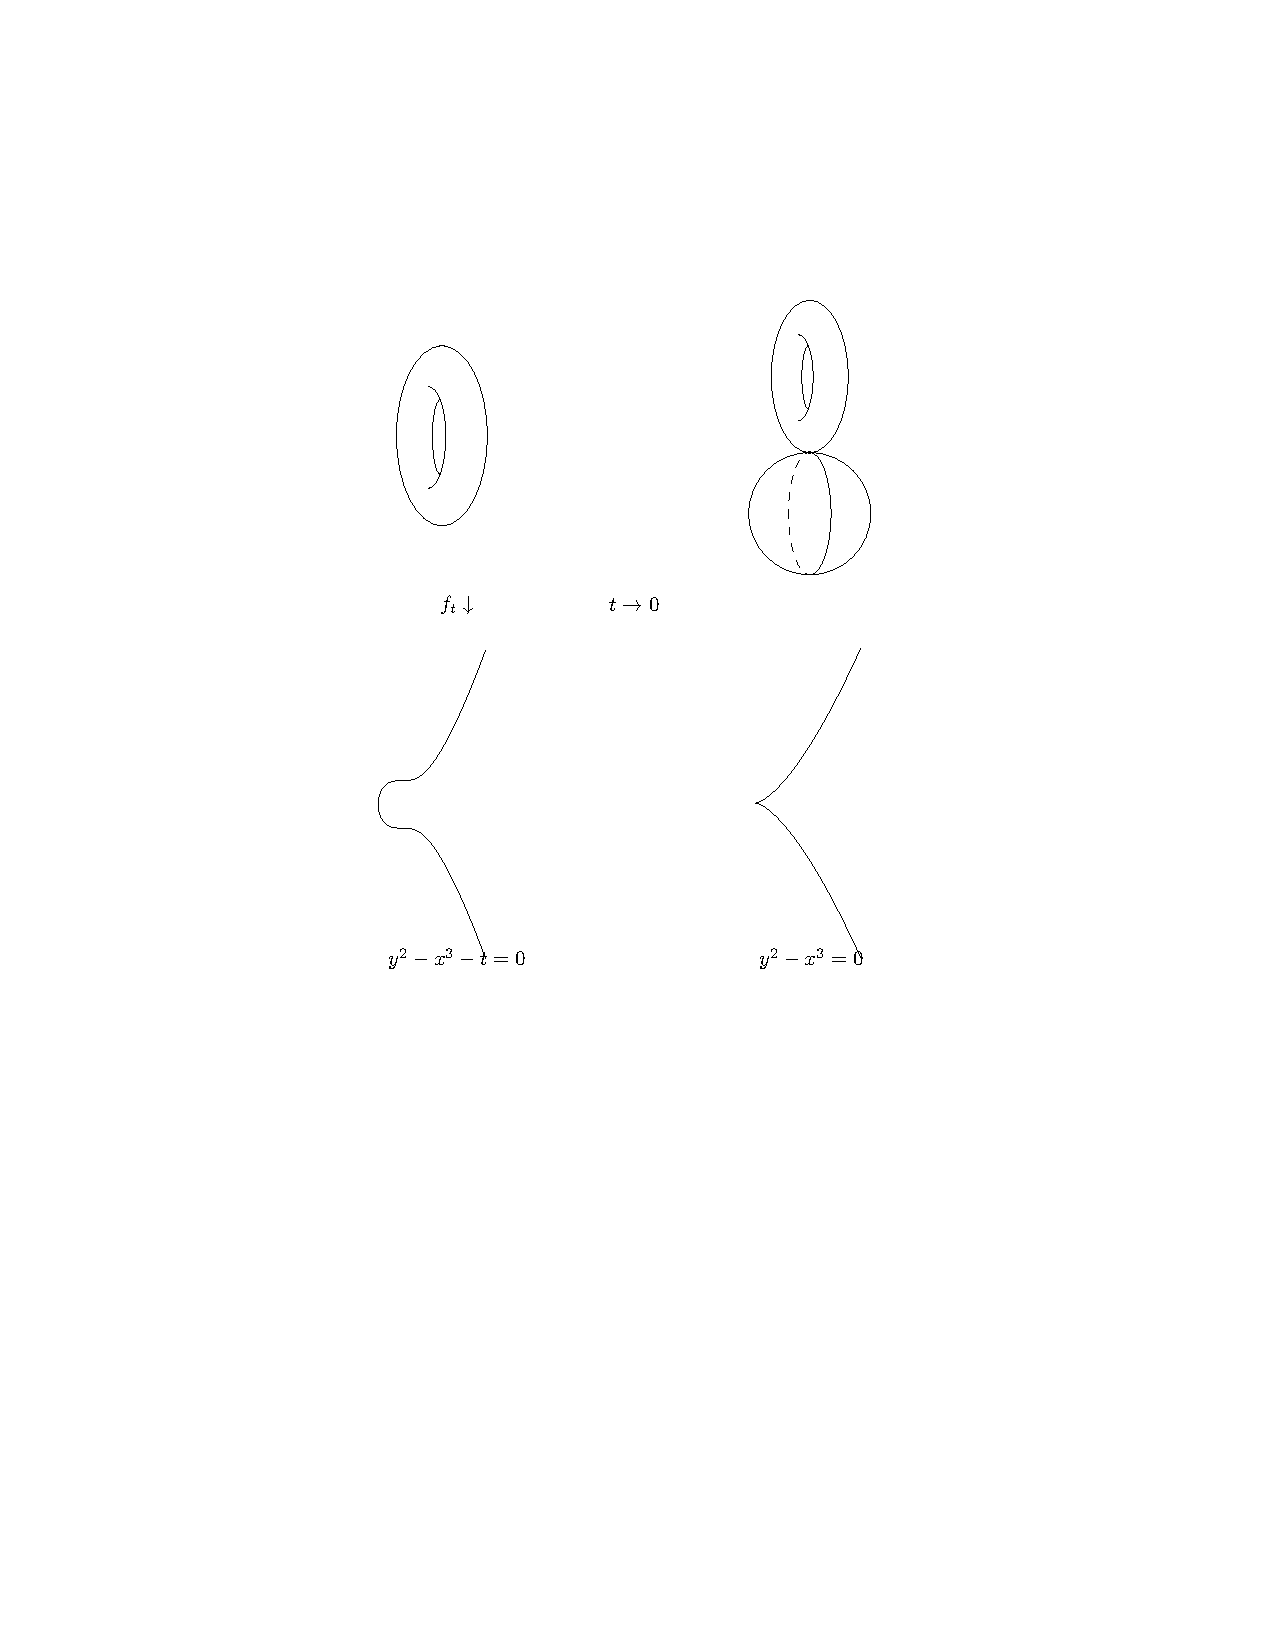
\includegraphics[width=0.6490\linewidth]{images/fig-3-1.pdf}
\caption{到 $\PP^2$ 的稳定映射族 $f_t$。当 $t\to0$ 时，亏格一的部分被收缩，像曲线因而出现尖点。}\label{fig:3.1}
\end{figure}
这归结为检查如下事项。对于 $\bar A=A/I$，其中 $I^2=0$，考虑
\Eq{3.4}{\begin{tikzcd}\Spec\bar A\arrow[r]\arrow[d]\&\overline{\mathcal M}_{0,k}(\PP^n)\arrow[d]\\\Spec A\arrow[r]\arrow[ur,dashed]\&\widetilde{\mathcal M}_{0,k}\end{tikzcd}.}
\SourcePage{44}
我们希望找到虚线箭头。换句话说，要找到
\Eq{3.5}{\begin{tikzcd}[row sep=2.3em,column sep=3em]\&\&X\\\bar C\arrow[rru,bend left=18,"{\bar f}"]\arrow[r,hook]\arrow[d]\&C\arrow[ur,dashed,"{\exists f?}"']\arrow[d]\\\Spec\bar A\arrow[r]\&\Spec A\end{tikzcd}}
中的 $f$：给定 $\bar f$，希望将其延拓。障碍类位于 $H^1(\bar C,\bar f^*\Theta_X)$ 中。在这里，$\bar f^*\Theta_{\PP^n}$ 在每个不可约分支 $\bar C'\subset\bar C$ 上整体生成，故有
\Eq{3.6}{0\longrightarrow K\longrightarrow\OO_{\bar C'}^{\oplus l}\longrightarrow\bar f^*\Theta_{\PP^n}|_{\bar C'}\longrightarrow0.}
在 $g=0$ 时，
\Eq{3.7}{0=H^1(\OO_{\bar C'})^{\oplus l}\longrightarrow H^1(\bar f^*\Theta_{\PP^n}|_{\bar C'})\longrightarrow H^2(K)=0.}

\end{proof}
\Lecture{12}{2019年10月8日}
\thmnum{theorem}{2}\begin{theorem}\label{thm:3.2}
若靶空间 $X$ 是射影概形，则 $\overline{\mathcal M}_{g,k}(X,\beta)$ 是固有、分离的 Deligne–Mumford 叠。
\end{theorem}
\begin{proof}
记 $\mathfrak m_{g,k}$ 为带 $k$ 个标记点的结点曲线的 Artin 叠。如果给定图表
\Eq{3.8}{\begin{tikzcd}C\arrow[r]\arrow[d]\&X\\T\arrow[u,bend left,"{\symbfit{x}}"]\end{tikzcd},}
这与下面的数据相同：
\Eq{3.9}{\begin{tikzcd}C\arrow[r]\arrow[d,"{\pi}"']\&X\times T\arrow[r]\arrow[d,"{\pr_2}"]\&X\arrow[d]\\T\arrow[r,equal]\arrow[u,bend left,"{\symbfit{x}}"]\&T\arrow[r]\&\mathrm{pt}\end{tikzcd}.}
它实际上是一个 $T$ 上的态射。无标记时，有万有曲线
\Eq{3.10}{\mathcal C_g\simeq\mathfrak m_{g,1}\longrightarrow\mathfrak m_g.}
因此，适当的带标记版本中，稳定映射叠嵌入相对 Hom 叠；无标记时记作
\Eq{3.11}{\overline{\mathcal M}_g(X)\hookrightarrow\Hom_{\mathfrak m_g}(\mathcal C_g,\mathfrak m_g\times X).}
右侧是一个局部有限型的 Artin 叠。由于稳定性为开条件，我们希望证明：
\thmnum{lemma}{3}\begin{lemma}\label{lem:3.3}稳定映射构成上述 Hom 叠的开子叠。\end{lemma}
\SourcePage{45}
\begin{figure}[H]\centering
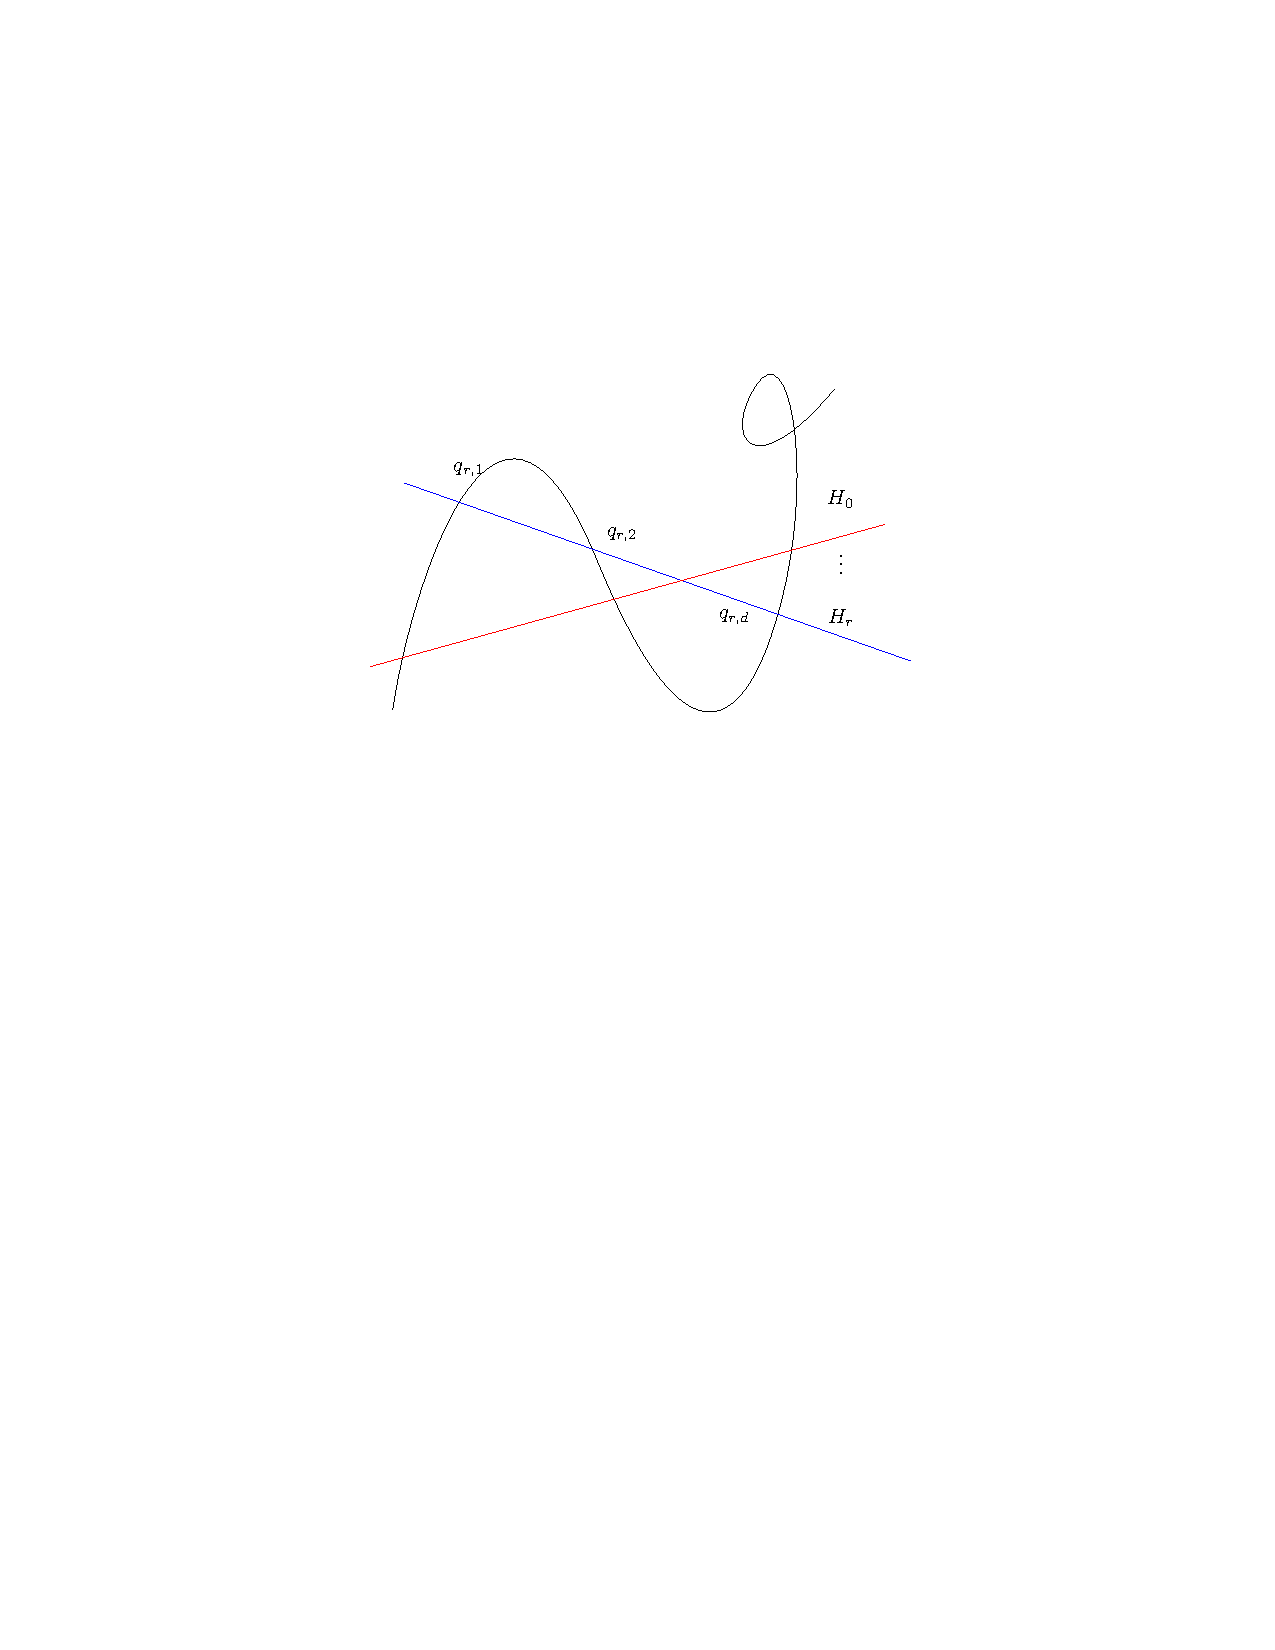
\includegraphics[width=0.6944\linewidth]{images/fig-3-2.pdf}
\caption{$\PP^r$ 中的 $r+1$ 个超平面与 $C_s$ 横截相交。}\label{fig:3.2}
\end{figure}
一旦固定 $\beta\in H_2(X,\ZZ)$，稳定映射只有有限多个“组合类型”。\footnote{这里指不可约分支的相交方式、各分支的亏格，以及每个分支的类 $\beta_i$，其中 $\beta=\sum_i\beta_i$。}这说明 $\overline{\mathcal M}_{g,k}(X,\beta)$ 拟紧。
更困难的部分是稳定约化，它给出分离性与固有性。Fulton 与 Pandharipande 的想法是：若 $X\subset\PP^r$，则有闭嵌入 $\overline{\mathcal M}(X,\beta)\hookrightarrow\overline{\mathcal M}(\PP^r,d)$，所以不妨取 $X=\PP^r$。关键在于
$L=\omega_{C/T}(\symbfit{x})\otimes f^*\OO_{\PP^r}(3)$ 对 $C/T$ 相对丰。因此，存在只依赖于 $g,k,d$ 的整数 $l$，使 $L^{\otimes l}$ 相对甚丰。
\end{proof}
考虑图 \ref{fig:3.2}。这些超平面 $H_i=(t_i=0)$，其中 $t_i\in\Gamma(\PP^r,\OO(1))$，在 $C$ 上给出额外标记点。于是，$\overline{\mathcal M}(\PP^r,d)$ 局部同构于刚化空间 $R$，其对象为
\Eq{3.12}{C\xrightarrow\pi T,\qquad\symbfit{q}=(q_{ij}),}
\SourcePage{46}
并满足一系列条件。定义
\Eq{3.13}{H_i=\OO_C(q_{i,1}+\cdots+q_{i,d}).}
对每个 $i$，要求
\Eq{3.14}{\pi^*\pi_*(H_i^{-1}\otimes H_0)\longrightarrow H_i^{-1}\otimes H_0}
为同构，并要求对所有 $i,j$ 都有 $H_i\simeq H_j$。还要给出 $\lambda_0,\ldots,\lambda_r:T\to\mathbb G_m$，用来调整 $H_i$ 的典范截面 $s_i$ 的尺度。
现在的想法，是在刚化后的层面进行稳定约化。
\section{超曲面的亏格零 Gromov–Witten 不变量}
设 $X\subset\PP^{n+1}$ 是次数为 $l$ 的超曲面，$X=Z(F)$。则 $\overline{\mathcal M}_0(X,d)\subset\overline{\mathcal M}_0(\PP^{n+1},d)$ 是一个向量丛截面的零点集。考虑万有图表
\Eq{3.15}{\begin{tikzcd}\mathcal C_0(\PP^{n+1})\arrow[r,"{f}"]\arrow[d,"{\pi}"']\&\PP^{n+1}\\\overline{\mathcal M}_0(\PP^{n+1})\end{tikzcd}.}
在几何纤维上，$f^*\OO(l)$ 在每个不可约分支上的次数都非负。$g=0$ 蕴含 $H^1(f_s^*\OO(l))=0$，因此基变换给出
\Eq{3.16}{R^1\pi_*f^*\OO(l)=0,}
而 $E=\pi_*f^*\OO(l)$ 局部自由。由 Riemann–Roch 定理，
\Eq{3.17}{\rank E=h^0(C_s,f_s^*\OO(l))=\deg f_s^*\OO(l)+(1-g)=dl+1.}
$F$ 定义一个截面 $\sigma\in\Gamma(\overline{\mathcal M}_0(\PP^{n+1}),E)$；在点 $(C_s,f_s)$ 上，$\sigma=0$ 当且仅当 $f_s(C_s)\subset X$。
\thmnum{definition}{2}\begin{definition}[Kontsevich]\label{def:3.2}
在环境模叠的 Chow 群中，\Term{xunijibenlei}{虚拟基本类}由下式表示：
\Eq{3.18}{[\overline{\mathcal M}_0(X,d)]^{\virt}:=c_{dl+1}(E)\cap[\overline{\mathcal M}_0(\PP^{n+1},d)].}
\end{definition}
注意，按照这个表示方式，
\Eq{3.19}{[\overline{\mathcal M}_0(X,d)]^{\virt}\in A_*(\overline{\mathcal M}_0(\PP^{n+1},d))\longrightarrow H_{2*}(\overline{\mathcal M}_0(\PP^{n+1},d)).}
首先，
\Eq{3.20}{\dim\overline{\mathcal M}_0(\PP^{n+1},d)=\deg f_s^*\Theta_{\PP^{n+1}}+(n+1)(1-g)-\underbrace{3}_{\dim\Aut(\PP^1)},}
\Eq{3.21}{=d(n+2)+n-2.}
对于 $n=3,l=5$，有 $\rank E=5d+1$，上述计算也给出
\Eq{3.22}{\dim\overline{\mathcal M}_0(\PP^4,d)=5d+1.}
\SourcePage{47}
\section{相交理论插叙}
文献 \cite{ref11} 是很好的参考书。设 $X$ 是域上的概形。考虑有限和
\Eq{3.23}{\sum_i n_i[V_i],}
其中 $V_i\subset X$ 是不可约、约化的闭子概形。\Term{youlidengjia}{有理等价}由如下数据生成：不可约子簇 $W\subset X$ 及非零有理函数 $f\in K(W)$。其除子定义为在余维一不可约子簇 $V\subset W$ 上的和：
\Eq{3.24}{[\operatorname{div}(f)]=\sum_{V\subset W}\operatorname{ord}_V(f)\,[V].}
现在定义 $X$ 的基本类。写不可约分支分解为
\Eq{3.25}{|X|=\bigcup_iX_i,}
并定义
\Eq{3.26}{[X]=\sum_i m_i[X_i],}
其中 $m_i$ 是 $\OO_{X,\eta_i}$ 作为自身模的长度，$\eta_i$ 为 $X_i$ 的泛点。
\examnum{1}\begin{example}\label{ex:3.1}
取 $X=\Spec A$ 为一个加厚点，$\dim_kA<\infty$。对于 $M\in A\text{-}\mathrm{Mod}$，我们关心其长度 $l$。按照定义，取一个组成列 $0=M_0\subset M_1\subset\cdots\subset M_l=M$，其逐次商是简单模，即在这里为 $A/\mathfrak p_i$，其中 $\mathfrak p_i$ 是相应的素理想。
例如，取 $A=k[\epsilon]/(\epsilon^{k+1})$。$A$ 作为 $A$ 模的长度为 $k+1$，来自序列
\Eq{3.27}{(\epsilon^{k+1})=0\subset(\epsilon^k)\subset\cdots\subset(\epsilon)\subset A.}
一般地，对于剩余域为 $k$ 的 Artin 局部环，所得到的长度就是其 $k$ 向量空间维数。
\end{example}
\Term{chowqun}{Chow 群}为
\Eq{3.28}{A_*(X)=Z_*(X)/\sim_{\mathrm{rat}},\qquad *=0,1,2,\ldots.}
\examnum{2}\begin{example}\label{ex:3.2}
仿射空间中，除最高维外的 Chow 群都消失：$A_i(\mathbb A^n)=0$，$i\ne n$，而 $A_n(\mathbb A^n)=\ZZ$。
对于射影空间，
\Eq{3.29}{A_i(\PP^n)=\begin{cases}\ZZ,&i=0,\ldots,n,\\0,&\text{其他情形}.\end{cases}}
\end{example}
\Lecture{13}{2019年10月9日}
\UnnumberedSubsection{固有推前与平坦拉回}
我们先定义固有推前。设 $f:X\to Y$ 为固有态射。定义很简单：对于子簇 $V\subset X$，令 $W=f(V)_{\mathrm{red}}\subset Y$，它也是子簇。于是得到域扩张 $K(W)\hookrightarrow K(V)$。定义
\Eq{3.30}{f_*[V]=\begin{cases}0,&\dim W<\dim V,\\{[K(V):K(W)]}\,[W],&\dim W=\dim V.\end{cases}}
现在必须证明：
\thmnum{proposition}{4}\begin{proposition}\label{pro:3.4}
上述 $f_*[V]$ 的定义下降为 $f_*:A_*(X)\to A_*(Y)$。
\end{proposition}
\SourcePage{48}
接下来需要平坦拉回。设 $f:X\to Y$ 为相对维数 $n$ 的平坦态射。对于 $Y$ 中维数为 $k$ 的子簇 $V$，拉回后的支撑 $f^{-1}(V)_{\mathrm{red}}\subset X$ 是若干子簇的并。
\thmnum{definition}{3}\begin{definition}\label{def:3.3}$f^*[V]=[f^{-1}(V)]$。\end{definition}
然后证明，这一操作与有理等价相容。
\UnnumberedSubsection{切除}
现在考虑这一“同调”理论中的切除性质。设 $i:Y\hookrightarrow X$ 为闭嵌入，就有开嵌入 $j:X\setminus Y\hookrightarrow X$。映射 $j^*:A_*(X)\to A_*(X\setminus Y)$ 实际上是满射，其核为 $A_*(Y)$ 推前的像，但这一推前未必单射。因此得到正合序列
\Eq{3.31}{A_*(Y)\xrightarrow{i_*}A_*(X)\xrightarrow{j^*}A_*(X\setminus Y)\longrightarrow0.}
\begin{proof}
利用循环群上的正合序列
\Eq{3.32}{Z_k(Y)\longrightarrow Z_k(X)\longrightarrow Z_k(X\setminus Y)\longrightarrow0}
并模去有理等价。
\end{proof}
\UnnumberedSubsection{Weil 除子}
设 $X$ 为 $n$ 维概形，Weil 除子为
\Eq{3.33}{D=\sum_i m_iD_i\in Z_{n-1}(X).}
真正希望用来进行相交的，并非这些“同调”类，而是某种“上同调”类，即 Cartier 除子。对任意概形 $X$，先用开集 $U_\alpha$ 覆盖它，在总商环中取
\Eq{3.34}{f_\alpha\in R(U_\alpha)^\times.}
它们形如 $g/h$，其中 $h$ 非零因子。对于所有 $\alpha,\beta$，要求 $f_\alpha/f_\beta\in\OO^\times(U_\alpha\cap U_\beta)$。于是，Cartier 除子为 $\{(U_\alpha,f_\alpha)\}$，并给出可逆层 $\OO(D)$。
设 $X$ 纯 $n$ 维。Cartier 除子到 $A_{n-1}(X)$ 的映射，将
\Eq{3.35}{\{(U_\alpha,f_\alpha)\}\longmapsto\bigcup_\alpha[\operatorname{div}(f_\alpha)].}
我们用 $D\mapsto[D]$ 表示它。
\UnnumberedSubsection{Cartier 除子}
现在研究与 Cartier 除子的相交。给定 $D=\{(U_\alpha,f_\alpha)\}$ 及纯 $k$ 维子簇 $j:V\hookrightarrow X$，定义
\Eq{3.36}{D\cdot[V]=\begin{cases}[j^{-1}D],&V\not\subset\operatorname{Supp}D,\\{[C]},&C\text{ 为 }V\text{ 上满足 }\OO_V(C)\simeq\OO_X(D)|_V\text{ 的 Cartier 除子}.\end{cases}}
它定义了
\Eq{3.37}{D\cdot-:A_k(X)\longrightarrow A_{k-1}(X).}
\SourcePage{49}
\UnnumberedSubsection{第一 Chern 类与 Segre 类}
第一 Chern 类定义如下。设 $L$ 为线丛，写成 $L=\OO_X(D)$，其中 $D$ 为 Cartier 除子。定义
\Eq{3.38}{\begin{aligned}c_1(L):A_*(X)&\longrightarrow A_{*-1}(X),\\z=\sum_i m_i[z_i]&\longmapsto D\cdot z.\end{aligned}}
为了得到高阶 Chern 类，先定义向量丛 $E\to X$ 的 \Term{segrelei}{Segre 类}。记 $\mathcal E$ 为 $E$ 的截面层，$r$ 为其秩。于是
\Eq{3.39}{E=\Spec_X\Sym^\bullet\mathcal E^\vee,}
其中
\Eq{3.40}{\mathcal E^\vee=\Hom_{\OO_X}(\mathcal E,\OO_X).}
$E$ 中的直线构成射影丛
\Eq{3.41}{\PP(E)=\operatorname{Proj}_X\Sym^\bullet(\mathcal E^\vee).}
它带有线丛 $\OO_{\PP(E)}(1)$。态射
\Eq{3.42}{p:\PP(E)\longrightarrow X}
既固有又平坦，因此可以对它使用上述拉回和推前。对于 $i\ge0$，Segre 类是算子
\Eq{3.43}{s_i(E):A_k(X)\longrightarrow A_{k-i}(X),}
定义为
\Eq{3.44}{s_i(E)\cap\alpha:=p_*\bigl(c_1(\OO_{\PP(E)}(1))^{r+i-1}\cap p^*\alpha\bigr).}
现在希望得到 Segre 类的投影公式；它直接由 Cartier 除子的相应公式推出。设 $f:X\to Y$ 固有，$E\to Y$ 为向量丛，则
\Eq{3.45}{f_*\bigl(s_i(f^*E)\cap\alpha\bigr)=s_i(E)\cap f_*\alpha.}
\thmnum{corollary}{5}\begin{corollary}\label{cor:3.5}$s_0(E)=\id$。\end{corollary}
\begin{proof}
对一个子簇的嵌入 $i:V\hookrightarrow X$ 使用投影公式。只需对单个簇证明，因而不妨令 $V=X$。若 $k=\dim X$，则
\Eq{3.46}{s_0(E)\cap[X]=m[X],}
因为 $A_k(X)=\ZZ\cdot[X]$ 中没有其他生成元。因此只须求出 $m$。这可以局部计算；在局部平凡化下，
\Eq{3.47}{\PP(E)=X\times\PP^{r-1},}
且 $\OO_{\PP(E)}(1)$ 从 $\PP^{r-1}$ 拉回。又有
\Eq{3.48}{c_1(\OO_{\PP^{r-1}}(1))^{r-1}\cap[\PP^{r-1}]=[\mathrm{pt}]\in A_0(\PP^{r-1}),}
故 $m=1$。
\end{proof}
\SourcePage{50}
\UnnumberedSubsection{Chern 类}
现在由 Segre 类得到 \Term{chernlei}{Chern 类}。令
\Eq{3.49}{s_t(E)=\sum_{i\ge0}s_i(E)t^i\in\operatorname{End}(A_*(X))[[t]],}
并定义
\Eq{3.50}{c_t(E)=s_t(E)^{-1}.}
这里确实需要对所有 $i,j$ 都有 $s_is_j=s_js_i$。
接着有和公式：只要有正合序列
\Eq{3.51}{0\longrightarrow E'\longrightarrow E\longrightarrow E''\longrightarrow0,}
就有
\Eq{3.52}{c_t(E)=c_t(E')\,c_t(E'').}
\UnnumberedSubsection{Gysin 拉回}
设 $V$ 为纯 $k$ 维簇，$\iota:X\hookrightarrow Y$ 为余维 $d$ 的正则嵌入。这等价于说，其理想在局部由正则序列 $I=(a_1,\ldots,a_d)\subset A$ 生成；也就是说，对 $i=1,\ldots,d$，$a_i$ 在 $A/(a_1,\ldots,a_{i-1})$ 中不是零因子。考虑笛卡尔方块
\Eq{3.53}{\begin{tikzcd}W\arrow[r]\arrow[d,"{g}"']\&V\arrow[d,"{f}"]\\X\arrow[r,hook,"{\iota}"']\&Y.\end{tikzcd}}
对于嵌入 $X\hookrightarrow Y$ 的理想层 $\mathcal I$，$\mathcal I/\mathcal I^2$ 为秩 $d$ 的局部自由层，因而给出秩 $d$ 的向量丛。定义\Term{facong}{法丛}
\Eq{3.54}{N_{X/Y}=\Spec_X\Sym^\bullet(\mathcal I/\mathcal I^2).}
类似地，令 $\mathcal J$ 为 $W\hookrightarrow V$ 的理想层；此时 $\mathcal J/\mathcal J^2$ 未必局部自由。定义\Term{fazhui}{法锥}
\Eq{3.55}{C_{W/V}:=\Spec_W\bigoplus_{m\ge0}\mathcal J^m/\mathcal J^{m+1}\hookrightarrow N_{W/V}:=\Spec_W\Sym^\bullet(\mathcal J/\mathcal J^2).}
\thmnum{proposition}{6}\begin{proposition}\label{pro:3.6}若 $V$ 纯 $k$ 维，则 $C_{W/V}$ 也是纯 $k$ 维。\end{proposition}
接下来是一个基本构造。先记
\Eq{3.56}{s_0:W\longrightarrow C_{W/V}}
为零截面。已知有
\Eq{3.57}{C_{W/V}\hookrightarrow N_{W/V}\hookrightarrow g^*N_{X/Y},}
因而可以作如下定义。
\thmnum{definition}{4}\begin{definition}[Gysin 拉回]\label{def:3.4}
令 $E=g^*N_{X/Y}$，把法锥的循环类推前到 $E$，并定义
\Eq{3.58}{\iota^![V]:=s_0^*[C_{W/V}],}
其中 $s_0^*=(\pi^*)^{-1}$，而
\Eq{3.59}{\pi^*:A_{k-d}(W)\longrightarrow A_k(E).}
\end{definition}
\begin{Note}{3.1}从几何上说，应把这个操作理解为与零截面相交。下面的命题保证这一理解有意义。\end{Note}
\SourcePage{51}
\thmnum{proposition}{7}\begin{proposition}\label{pro:3.7}$\pi^*$ 为同构。\end{proposition}
\begin{proof}满射性容易，由切除性质推出；单射性较难。\end{proof}
这套构造可以概括为：取 $C_{W/V}$，将它嵌入 $g^*N_{X/Y}$，最后与零截面相交。以上先针对单个簇 $V$ 说明。
\Lecture{14}{2019年10月15日}
考虑图式
\Eq{3.60}{Z\overset{\iota}{\hookrightarrow}Y\xleftarrow{f}X,}
其中 $\iota$ 为局部完全交嵌入。设 $W\subset X$ 为 $d$ 维子簇。得到
\Eq{3.61}{\begin{tikzcd}W_Z\arrow[r]\arrow[d]\&W\arrow[d,hook]\\X_Z\arrow[r]\arrow[d,"{g}"']\&X\arrow[d,"{f}"]\\Z\arrow[r,hook,"{\iota}"']\&Y.\end{tikzcd}}
此时
\Eq{3.62}{C_{W_Z/W}=\Spec_{W_Z}\bigoplus_{m\ge0}\mathcal I^m/\mathcal I^{m+1}}
纯 $d$ 维。拉回法丛，便有
\Eq{3.63}{C_{W_Z/W}\hookrightarrow g^*N_{Z/Y}|_{W_Z}.}
于是
\Eq{3.64}{\iota^![W]:=s_0^*[C_{W_Z/W}]\in A_{d-c}(W_Z)\longrightarrow A_{d-c}(X_Z),}
其中 $c$ 为 $\iota$ 的余维，最后一个箭头为推前。
为什么要用法锥？这里有一个称为\Term{xiangfazhuibianxing}{形变到法锥}的构造。\footnote{严格说来，这应称为退化，但大家都称它为变形。}考虑 $M:=\operatorname{Bl}_{X\times\{0\}}(Y\times\mathbb A^1)$。在 $t\in\mathbb A^1\setminus\{0\}$ 上，仍是 $X\hookrightarrow Y$；在 $t=0$ 上则有
\Eq{3.65}{X\hookrightarrow C_{X/Y}\hookrightarrow\PP(C_{X/Y}\oplus\mathbb A^1)\cup\operatorname{Bl}_X Y.}
关键在于：对于在平坦族中表现良好、又只依赖 $X$ 附近局部情况的问题，例如相交重数，$X\hookrightarrow Y$ 可以用 $X\hookrightarrow C_{X/Y}$ 代替。
现在给出一个应用。设 $X=Z(f)\subset\PP^{n+1}$，$\deg f=l$。我们想计算 $\mathcal M_0(X)$ 的\Term{xunijibenlei}{虚拟基本类}。回忆万有曲线
$\mathcal M_0(\PP^{n+1})\xleftarrow{\pi}\mathcal C\xrightarrow{\phi}\PP^{n+1}$，以及秩 $r$ 的向量丛
\Eq{3.66}{E=\pi_*\phi^*\OO(l)\longrightarrow\mathcal M_0(\PP^{n+1})=:M,}
称为变形丛。多项式 $f$ 定义了截面 $s\in\Gamma(E)$，其零点概形为 $(s=0)=\mathcal M_0(X)\subset\mathcal M_0(\PP^{n+1})$。现在将 $\im(s)$ 与零截面相交：
\Eq{3.67}{\begin{tikzcd}\mathcal M_0(X)\arrow[r]\arrow[d]\&M\arrow[d,"{s}"]\\M\arrow[r,"{s_0}"']\&E.\end{tikzcd}}
\SourcePage{52}
得到
\Eq{3.68}{s_0^![M]\in A_{\dim M-r}(\mathcal M_0(X)).}
\section{障碍理论与虚拟基本类}
\subsection{基本思想}
这一思想来自文献~\cite{ref21}。在局部，例如 $U\subset M$ 上，将 $U$ 嵌入光滑空间 $V$，对应于 $V$ 上的理想层 $\mathcal I$。有图式
\Eq{3.69}{\begin{tikzcd}C_{U/V}=\Spec_U\bigoplus_{m\ge0}\mathcal I^m/\mathcal I^{m+1}\arrow[r,hook]\&N_{U/V}=\Spec_U\Sym^\bullet(\mathcal I/\mathcal I^2)\\\&T_V|_U=\Spec_U\Sym^\bullet(\Omega_V|_U)\arrow[u,"{\text{作用}}"'].\end{tikzcd}}
注意，$T_V|_U$ 的加法作用保持 $C_{U/V}$ 不变。
现在希望将 $N_{U/V}\hookrightarrow E_1$ 嵌入某个向量丛，并把构造整体化；其中要处理的正是 $T_V|_U$ 在 $C_{U/V}$ 上的作用。粘合所需的数据如下：对于
\Eq{3.70}{\begin{tikzcd}T_V|_U\arrow[r]\arrow[d]\&E_0\arrow[d]\\N_{U/V}\arrow[r]\&E_1,\end{tikzcd}}
得到序列
\Eq{3.71}{T_V|_U\longrightarrow E_0\oplus N_{U/V}\longrightarrow E_1\longrightarrow0,}
并要求它正合。
实现相容性主要有两种方法。第一种是文献~\cite{ref21} 中 Artin 风格的障碍理论；另一种是文献~\cite{ref3} 所用的余切复形与导出范畴方法。我们采用第二种。
\subsection{关于余切复形的补充}
对于 $f:X\to Y$，有正合序列
\Eq{3.72}{f^*\Omega_Y\longrightarrow\Omega_X\longrightarrow\Omega_{X/Y}\longrightarrow0.}
当 $f$ 光滑时，箭头 $f^*\Omega_Y\to\Omega_X$ 为单射。一般情况下，需要把 $\Omega_{X/Y}$、$\Omega_X$ 等替换为拟凝聚层的复形 $L^\bullet_{X/Y}$、$L^\bullet_X$ 等。导出范畴中有
\Eq{3.73}{\cdots\longrightarrow Lf^*L_Y^\bullet\longrightarrow L_X^\bullet\longrightarrow L_{X/Y}^\bullet\longrightarrow Lf^*L_Y^\bullet[1]\longrightarrow L_X^\bullet[1]\longrightarrow\cdots,}
也就是说，这给出一个正合三角。它延伸了最初的序列，因为
\Eq{3.74}{\begin{aligned}h^{-1}(L_{X/Y}^\bullet)&\longrightarrow\underbrace{h^0(Lf^*L_Y^\bullet)}_{f^*\Omega_Y}\longrightarrow\underbrace{h^0(L_X^\bullet)}_{\Omega_X}\\&\longrightarrow\underbrace{h^0(L_{X/Y}^\bullet)}_{\Omega_{X/Y}}\longrightarrow\underbrace{h^1(Lf^*L_Y^\bullet)}_{0}.\end{aligned}}
现在定义范畴 $\DQCoh(\OO_X)$。它的对象为复形
\Eq{3.75}{\cdots\longrightarrow \mathcal F^{-2}\xrightarrow{d_{\mathcal F}^{-2}}\mathcal F^{-1}\xrightarrow{d_{\mathcal F}^{-1}}\mathcal F^0\longrightarrow\cdots,}
其中微分记为
\Eq{3.76}{d^\bullet=d_{\mathcal F}^\bullet:\mathcal F^\bullet\longrightarrow \mathcal F^\bullet[1].}
\SourcePage{53}
先取复形的态射 $\phi^\bullet:\mathcal F^\bullet\to \mathcal G^\bullet$，并模去同伦：$\phi^\bullet\simeq\psi^\bullet$ 当且仅当存在 $h^\bullet:\mathcal F^\bullet\to \mathcal G^\bullet[-1]$，使得
\Eq{3.77}{\phi^\bullet-\psi^\bullet=d_{\mathcal G}^\bullet\circ h^\bullet+h^\bullet\circ d_{\mathcal F}^\bullet.}
然后进行局部化，使拟同构可逆。因此，$\DQCoh(\OO_X)$ 中的一个态射 $\mathcal F^\bullet\to \mathcal G^\bullet$ 可用屋顶图式表示：
\Eq{3.78}{\begin{tikzcd}\&\widetilde{\mathcal F}^\bullet\arrow[dl,"{\psi^\bullet}"',"{\sim}"]\arrow[dr,"{\widetilde\phi^\bullet}"]\&\\\mathcal F^\bullet\arrow[rr,dashed,"{\phi^\bullet}"']\&\&\mathcal G^\bullet.\end{tikzcd}}
再考虑导出函子。给定 $f:X\to Y$，希望定义 $Rf_*$。将 $\mathcal F^\bullet$ 换成一个与之拟同构、适于计算导出函子的内射分解 $\mathcal I_{\mathcal F}^\bullet$；为每个 $\mathcal F^\bullet$ 选定一个这样的分解。定义
\Eq{3.79}{Rf_*\mathcal F^\bullet:=f_*\mathcal I_{\mathcal F}^\bullet.}
\begin{Note}{3.2}左导出张量积 $\otimes^L$ 与拉回 $Lf^*=f^{-1}(-)\otimes^L_{f^{-1}\OO_Y}\OO_X$ 较为微妙，但同样可以构造。\end{Note}
余切复形的构造如下。先考虑仿射情形。给定环同态 $\phi:A\to B$，可以将 $B$ 作为 $A$-代数作自由分解，而且可以典范地完成。得到增广单纯代数分解 $P_\bullet\to B$，其各项形如
\Eq{3.80}{P_\bullet=[\cdots\longrightarrow A[A[B]]\longrightarrow A[B]].}
在这种情况下，
\Eq{3.81}{L_{B/A}^\bullet=\Omega_{P_\bullet/A}\otimes_{P_\bullet}B,}
即相应复形的第 $-n$ 项为
\Eq{3.82}{L^{-n}_{B/A}=\Omega_{P_n/A}\otimes_{P_n}B.}
对于代数叠的态射 $X\to Y$，也可以对 $f^{-1}\OO_Y\to\OO_X$ 作类似的“单纯”分解。更多内容可参阅文献~\cite{ref19} 或 Stacks Project。
下面这一点很重要。在局部可以嵌入一个相对光滑的空间：
\Eq{3.83}{\begin{tikzcd}X\arrow[rr,hook,"{\iota}"]\arrow[dr,"{f}"']\&\&Z\arrow[dl,"{\text{光滑}}"]\\\&Y.\&\end{tikzcd}}
记 $\mathcal I=\mathcal I_{X/Z}$，则
\Eq{3.84}{\tau_{\ge-1}L_{X/Y}^\bullet=\bigl[\mathcal I/\mathcal I^2\longrightarrow\underbrace{\Omega_{Z/Y}|_X}_{\iota^*\Omega_{Z/Y}}\bigr],}
两项分别位于次数 $-1$ 与 $0$。也就是说，在对应的线性纤维空间层面，得到
\Eq{3.85}{[T_{Z/Y}|_X\longrightarrow N_{X/Z}],}
这正是将 $C_{X/Z}\hookrightarrow N_{X/Z}$ 整体化所需要的数据。
\SourcePage{54}
\subsection{Behrend--Fantechi 的定义}
\thmnum{definition}{5}\begin{definition}[完美障碍理论]\label{def:3.5}
设 $f:X\to Y$ 为代数叠的态射，且 $X$ 为 Deligne--Mumford 叠。$X/Y$ 上的\Term{wanmeizhangaililun}{完美障碍理论}，由局部自由凝聚层的两项复形 $\mathcal F^\bullet=[\mathcal F^{-1}\to \mathcal F^0]$ 以及 $\DQCoh(\OO_X)$ 中的态射
\Eq{3.86}{\phi^\bullet:\mathcal F^\bullet\longrightarrow L_{X/Y}^\bullet}
组成，并满足：
\begin{enumerate}
\item $h^0(\phi^\bullet)$ 为同构；
\item $h^{-1}(\phi^\bullet)$ 为满射。
\end{enumerate}
\end{definition}
\Lecture{15}{2019年10月17日}
关键是如下构造。在局部将 $X$ 嵌入一个在 $Y$ 上光滑的空间 $Z$：
\Eq{3.87}{\begin{tikzcd}X\arrow[rr,hook]\arrow[dr,"{f}"']\&\&Z\arrow[dl]\\\&Y.\&\end{tikzcd}}
假设 $\phi^\bullet$ 可由真正的复形态射表示。已经知道 $\tau_{\ge-1}L_{X/Y}^\bullet=[\mathcal I/\mathcal I^2\to\Omega_{Z/Y}|_X]$，所以得到交换图
\Eq{3.88}{\begin{tikzcd}\mathcal F^{-1}\arrow[r]\arrow[d]\&\mathcal I/\mathcal I^2\arrow[d]\\\mathcal F^0\arrow[r]\&\Omega_{Z/Y}|_X.\end{tikzcd}}
它给出复形
\Eq{3.89}{0\longrightarrow \mathcal F^{-1}\longrightarrow \mathcal F^0\oplus\mathcal I/\mathcal I^2\longrightarrow\Omega_{Z/Y}|_X\longrightarrow0.}
可以分别考察各项处的正合性。在第一项处正合，等价于 $h^{-1}(\phi^\bullet)$ 单射；在第二项处正合，等价于 $h^{-1}(\phi^\bullet)$ 满射且 $h^0(\phi^\bullet)$ 单射；在第三项处正合，等价于 $h^0(\phi^\bullet)$ 满射。完美障碍理论定义中的条件保证，对偶后的线性纤维空间序列
\Eq{3.90}{0\longrightarrow T_{Z/Y}|_X\longrightarrow F_0\oplus N_{X/Z}\longrightarrow F_1}
正合，其中 $F_i=L(\mathcal F^{-i})=\Spec_X\Sym^\bullet \mathcal F^{-i}$。
\thmnum{lemma}{8}\begin{lemma}\label{lem:3.8}
\begin{enumerate}[label=(\alph*)]
\item 存在唯一的锥 $C_{\phi^\bullet}\subset F_1$，使得
\Eq{3.91}{0\longrightarrow T_{Z/Y}|_X\longrightarrow F_0\oplus C_{X/Z}\longrightarrow C_{\phi^\bullet}\longrightarrow0}
正合。
\item $C_{\phi^\bullet}$ 与 $Z$ 的选择无关，并且在复形同伦下不变。
\end{enumerate}
\end{lemma}
\begin{proof}
(a) 利用局部自由性，将\eqref{eq:3.90}中的序列局部分裂，结论便显然成立。
\SourcePage{55}
(b) 对两个选择 $Z$ 与 $Z'$，取它们在 $Y$ 上的共同光滑加细，便归结为如下比较图：
\Eq{3.92}{\begin{tikzcd}X\arrow[rr]\arrow[dr]\arrow[ddr]\&\&Z'\arrow[dl,"{\text{光滑}}"]\\\&Z\arrow[d]\&\\\&Y.\&\end{tikzcd}}

\end{proof}
上面给出了粘合的图景。文献~\cite{ref3} 有更内蕴的叙述；如果愿意使用 Artin 叠，这并不困难。定义
\Eq{3.93}{\mathcal M_{X/Y}=[N_{X/Z}/T_{Z/Y}|_X],}
称为\Term{neiyunfaceng}{内蕴法层}；同时定义\Term{neiyunfazhui}{内蕴法锥}
\Eq{3.94}{\mathcal C_{X/Y}=[C_{X/Z}/T_{Z/Y}|_X].}
在绝对情形中，它为纯 $0$ 维。
复形 $\mathcal F^\bullet$ 也给出一个叠
\Eq{3.95}{h^0/h^1(\mathcal F^\bullet)=[F_1/F_0].}
于是，$\phi^\bullet:\mathcal F^\bullet\to L_{X/Y}^\bullet$ 为完美障碍理论，当且仅当
\Eq{3.96}{\mathcal M_{X/Y}\hookrightarrow h^0/h^1(\mathcal F^\bullet)}
为单态射。在这种情况下，通过笛卡尔图式构造 $C_{\phi^\bullet}$：
\Eq{3.97}{\begin{tikzcd}C_{\phi^\bullet}\arrow[rr,hook]\arrow[d]\&\&F_1\arrow[d]\\\mathcal C_{X/Y}\arrow[r,hook]\&\mathcal M_{X/Y}\arrow[r,hook]\&h^0/h^1(\mathcal F^\bullet).\end{tikzcd}}
为什么称其为障碍理论？照例考虑提升问题。取平方为零的扩张 $T\hookrightarrow\overline T$，即理想层 $\mathcal I=\mathcal I_{T/\overline T}$ 满足 $\mathcal I^2=0$。考虑图式
\Eq{3.98}{\begin{tikzcd}[row sep=2.5em,column sep=3em]T\arrow[r,"{h}"]\arrow[d,hook,"{\iota}"']\&X\arrow[d,"{f}"]\\\overline T\arrow[r,"{g}"']\arrow[ur,dashed,"{\exists\,\widetilde g?}"]\&Y.\end{tikzcd}}
$L_{X/Y}^\bullet$ 的函子性给出
\Eq{3.99}{\begin{aligned}\operatorname{Ob}(h)&:=\bigl[Lh^*L_{X/Y}^\bullet\longrightarrow L_{T/\overline T}^\bullet\longrightarrow\underbrace{\tau_{\ge-1}L_{T/\overline T}^\bullet}_{\mathcal I[1]}\bigr]\\&\in\Ext^1(Lh^*L_{X/Y}^\bullet,\mathcal I).\end{aligned}}
\begin{custom}{事实 2}\hypertarget{fact:2}{}
$\operatorname{Ob}(h)=0$ 当且仅当提升 $\widetilde g$ 存在。此时，提升在同构意义下构成一个 $\Ext^0(Lh^*L_{X/Y}^\bullet,\mathcal I)$-挠子。
\end{custom}
\SourcePage{56}
\thmnum{proposition}{9}\begin{proposition}[\cite{ref3}]\label{pro:3.9}
$\phi^\bullet:\mathcal F^\bullet\to L_{X/Y}^\bullet$ 为完美障碍理论，当且仅当对于所有上述提升问题，相应的第一条件也适用于
\Eq{3.100}{\phi^*\operatorname{Ob}(h)\in\Ext^1(\underbrace{h^*\mathcal F^\bullet}_{Lh^*\mathcal F^\bullet},\mathcal I),}
即该类为零当且仅当提升存在；而相应的第二条件适用于 $\Ext^0(h^*\mathcal F^\bullet,\mathcal I)$，即提升在同构意义下构成这一群的挠子。这也等价于
\Eq{3.101}{\mathcal M_{X/Y}\longrightarrow[F_1/F_0]=h^0/h^1(\mathcal F^\bullet)}
为嵌入。
\end{proposition}
\thmnum{theorem}{10}\begin{theorem}\label{thm:3.10}
$\mathcal M_{X/Y}$ 是泛的、最小的“障碍理论”；除非 $X/Y$ 为局部完全交，否则它一般不是向量丛叠。$\mathcal F^\bullet\to L_{X/Y}^\bullet$ 给出将它嵌入向量丛叠 $[F_1/F_0]$ 的嵌入。
\end{theorem}
虚拟基本类为
\Eq{3.102}{[X]^{\virt,\phi^\bullet}:=s_0^![C_{\phi^\bullet}]\in A_*(X),}
其中 $s_0:X\to F_1$ 为零截面。
\subsection{Gromov--Witten 理论的障碍理论}
\begin{Warning}{3.1}现在 $X$ 表示目标空间，与上一小节的 $X$ 含义不同。\end{Warning}
记 $M=\mathcal M_{g,k}(X,\beta)$，并相应记 $\mathfrak m=\mathfrak m_{g,k}$。前者为到 $X$ 的稳定映射的模叠，源曲线的亏格为 $g$，带 $k$ 个标记点，且 $\beta\in H_2(X,\ZZ)$。
现在要为 Gromov--Witten 理论构造 $\phi^\bullet:\mathcal F^\bullet\to L^\bullet$。我们相对于 Artin 叠 $\mathfrak m$ 工作，考虑 $M/\mathfrak m$。有泛图式
\Eq{3.103}{\begin{tikzcd}\&X\&\\\mathcal C\arrow[ur,"{f}"]\arrow[rr]\arrow[d,"{\pi}"']\&\&\overline{\mathcal C}\arrow[d]\\M\arrow[rr]\arrow[u,bend left=40,"{x}"]\&\&\mathfrak m,\end{tikzcd}}
其中方块为笛卡尔方块。考虑位于次数 $-1$ 与 $0$ 的复形
\Eq{3.104}{\omega_\pi=[\omega_{\mathcal C/M}\longrightarrow0].}
有
\Eq{3.105}{f^*\Omega_X=Lf^*L_X^\bullet\longrightarrow L_{\mathcal C}^\bullet\longrightarrow L_{\mathcal C/\overline{\mathcal C}}^\bullet=\pi^*L_{M/\mathfrak m}^\bullet,}
其中使用了 $\overline{\mathcal C}/\mathfrak m$ 的平坦性。施加 $R\pi_*(-\otimes\omega_\pi)$，并用迹映射，得到
\Eq{3.106}{\begin{aligned}\phi^\bullet:R\pi_*(f^*\Omega_X\otimes\omega_\pi)&\longrightarrow R\pi_*(\pi^*L_{M/\mathfrak m}^\bullet\otimes\omega_\pi)\\&\simeq L_{M/\mathfrak m}^\bullet\otimes^L R\pi_*\omega_\pi\xrightarrow{\id\otimes\operatorname{tr}}L_{M/\mathfrak m}^\bullet,\end{aligned}}
其中 $\operatorname{tr}:R\pi_*\omega_\pi\to\OO_M$。因此还须证明：
\thmnum{lemma}{11}\begin{lemma}\label{lem:3.11}
$R\pi_*(f^*\Omega_X\otimes\omega_\pi)$ 拟同构于局部自由层的两项复形 $[\mathcal F^{-1}\to \mathcal F^0]$。
\end{lemma}
\SourcePage{57}
\begin{proof}
线丛
\Eq{3.107}{L:=\omega_{\mathcal C/M}(x)\otimes f^*(\OO_X(1))^{\otimes3}}
对 $\mathcal C/M$ 相对丰。记 $\mathcal E:=f^*\Omega_X\otimes\omega_{\mathcal C/M}$。当 $N\gg0$ 时，
\begin{itemize}
\item $\pi^*\pi_*(\mathcal E\otimes L^{\otimes N})\to\mathcal E\otimes L^{\otimes N}$ 为满射；
\item $R^1\pi_*(\mathcal E\otimes L^{\otimes N})=0$；
\item 对每个几何点 $s\to M$，都有 $H^0(\mathcal C_s,L_s^{\otimes(-N)})=0$。
\end{itemize}
定义
\Eq{3.108}{\mathcal F:=\pi^*\pi_*(\mathcal E\otimes L^{\otimes N})\otimes L^{\otimes(-N)}.}
它确实是向量丛。令 $\mathcal H=\ker(\mathcal F\twoheadrightarrow\mathcal E)$，就得到向量丛的正合序列
\Eq{3.109}{0\longrightarrow\mathcal H\longrightarrow\mathcal F\longrightarrow\mathcal E\longrightarrow0.}
注意
\Eq{3.110}{H^0(\mathcal C_s,\mathcal F_s)=H^0\bigl(\mathcal C_s,\pi_s^*(\pi_*(\mathcal E\otimes L^{\otimes N}))_s\otimes L_s^{\otimes(-N)}\bigr),}
因此
\Eq{3.111}{H^0(\mathcal C_s,\mathcal F_s)=\underbrace{H^0(\mathcal C_s,L_s^{\otimes(-N)})}_{0}\otimes(\pi_*(\mathcal E\otimes L^{\otimes N}))_s=0.}
这说明 $\pi_*\mathcal F=0$，从而 $\pi_*\mathcal H=0$。于是 $R^1\pi_*\mathcal F$ 和 $R^1\pi_*\mathcal H$ 局部自由。由 \eqref{eq:3.109} 得到
\Eq{3.112}{R\pi_*(\mathcal E[1])\simeq[R^1\pi_*\mathcal H\longrightarrow R^1\pi_*\mathcal F],}

\end{proof}
\subsection{Gromov--Witten 不变量}
设 $X$ 光滑，$\dim X=n$。固定 $g$、$k$ 和 $\beta$，得到
\Eq{3.113}{[\mathcal M_{g,k}(X,\beta)]^{\virt,\phi^\bullet}\in A_d(\mathcal M_{g,k}(X,\beta)).}
这一类在 $X$ 的变形下不变。其维数具体为
\Eq{3.114}{d=\underbrace{3g-3+k}_{\dim\mathfrak m_{g,k}}+c_1(X)\cdot\beta+n(1-g),}
后两项来自秩 $n$ 向量丛的 Riemann--Roch 公式，且 $\deg f_s^*\Theta_X=c_1(X)\cdot\beta$。也就是说，
\Eq{3.115}{d=c_1(X)\cdot\beta+(n-3)(1-g)+k.}
它称为\Term{yuqiweishu}{预期维数}；对于 $\phi^\bullet:\mathcal F^\bullet\to L_{X/Y}^\bullet$，它等于 $\rank F_0-\rank F_1+\dim Y$。
对于 Calabi--Yau 三维簇，$n=3$、$k=0$，所以 $d=0$。
\Lecture{16}{2019年10月22日}
\SourcePage{58}
对于其他情形，有两个自然映射：
\Eq{3.116}{\begin{aligned}\operatorname{ev}:\mathcal M_{g,k}(X,\beta)&\longrightarrow\underbrace{X\times\cdots\times X}_{k\text{ 个}},\\(C,x=(x_1,\ldots,x_k),f)&\longmapsto(f(x_1),\ldots,f(x_k)),\\p:\mathcal M_{g,k}(X,\beta)&\longrightarrow\overline{\mathcal M}_{g,k},\\(C,x,f)&\longmapsto(C,x)^{\mathrm{st}}.\end{aligned}}
这里 $\overline{\mathcal M}_{g,k}$ 为稳定曲线的 Deligne--Mumford 叠；忘却映射后作稳定化，要求 $2g-2+k>0$。
这样便得到 Gromov--Witten 不变量。对于 $\alpha_1,\ldots,\alpha_k\in H^*(X)$ 和 $\gamma\in H^*(\overline{\mathcal M}_{g,k})$，定义
\Eq{3.117}{\int_{[\mathcal M_{g,k}(X,\beta)]^{\virt}}\operatorname{ev}^*(\alpha_1\times\cdots\times\alpha_k)\smile p^*\gamma=:\langle\alpha_1,\ldots,\alpha_k;\gamma\rangle_{\GW}^{g,k,\beta}.}
\subsection{Gromov--Witten 不变量的变形不变性}
考虑固有光滑簇的族
\Eq{3.118}{q:\mathcal X\longrightarrow S.}
我们希望比较各纤维的 Gromov--Witten 理论，直观上希望说它们相同。
给定 $\beta\in H_2(X_s,\ZZ)$，沿基底中的路径平行移动，便在其他纤维 $H_2(X_{s'},\ZZ)$ 中得到类；它在单值变换的意义下确定。记 $\iota_s:X_s\hookrightarrow\mathcal X$。取这一类对应的相对稳定映射模叠 $M$，其映射到总空间后的曲线类为 $(\iota_s)_*\beta$，则有
\Eq{3.119}{\begin{tikzcd}M_s\arrow[r]\arrow[d]\&M\arrow[d]\\s\arrow[r,hook,"{j_s}"']\&S.\end{tikzcd}}
拉回虚拟类，得到
\Eq{3.120}{[M_s]^{\virt}:=j_s^![M]^{\virt}.}
\thmnum{proposition}{12}\begin{proposition}\label{pro:3.12}
若 $S$ 是局部完全交（例如光滑），并且 $s,s'$ 属于同一连通分支，则推前到 $A_*(M)$ 的类满足代数等价
\Eq{3.121}{[M_s]^{\virt}\sim[M_{s'}]^{\virt}.}
特别地，在曲线类和插入类作相应平行移动后，$X_s$ 与 $X_{s'}$ 的 Gromov--Witten 不变量相同。
\end{proposition}
